%++++++++++++++++++++++++++++++++++++++++
\documentclass[letterpaper,12pt]{article}
\usepackage{tabularx} % extra features for tabular environment
\usepackage{amsmath}  % improve math presentation
\usepackage{graphicx} % takes care of graphic including machinery
\usepackage[margin=1in,letterpaper]{geometry} % decreases margins
\usepackage{cite} % takes care of citations
\usepackage{float}
\usepackage{subfig}
\usepackage[final]{hyperref} % adds hyper links inside the generated pdf file
\usepackage[parfill]{parskip}
\hypersetup{
	colorlinks=true,       % false: boxed links; true: colored links
	linkcolor=blue,        % color of internal links
	citecolor=blue,        % color of links to bibliography
	filecolor=magenta,     % color of file links
	urlcolor=blue         
}
%++++++++++++++++++++++++++++++++++++++++

\begin{document}

\title{Efficient Realistic Human Skin Rendering}
\author{Ke Wang \space\space\space kwang82@ucsc.edu}
\date{}
\maketitle

\begin{abstract}
Human skin rendering is categorized as a high albedo media rendering problem, which is traditionally hard to render with regard to efficiency and accuracy using Monte Carlo volumetric path tracing. Both subsurface scattering Photon Beam Diffusion (PBD)\cite{habel2013photon} and Sum of Exponentials (SoE)\cite{christensen2015approximate} methods address the accuracy and efficiency problem. GPGPU computing is able to achieve a huge rendering efficiency gain but the subsurface scattering sampling method used in CPU can not be immigrated to GPU naively since GPGPU computing has different computing model and limitations with CPU computing. I devised a novel sampling method for GPU based subsurface scattering and implemented both PBD and SoE in CUDA, Nvidia's GPGPU programming language\cite{han2011hicuda}. I tested well-known CPU based renderer pbrt-v3\cite{pharr2016physically}, my GPU PBD and my GPU SoE with three elaborately chosen scenes and showed that my implementations achieved both efficiency and accuracy, which proves that my GPU PBD and GPU SoE are able to produce efficient realistic human skin rendering.
\end{abstract}

\section{Introduction}
Human skin rendering is an interesting topic in rendering and it's generally hard to render realistic looking human skin. One can easily identify that a human face rendering is fake by comparing with real human face. First, traditional rendering methods focus on surface. The studies observe and formulate how light bounces on object surface as \textit{BRDF (Bidirectional Reflectance Distribution Function)}. For example, matte painting is rough so the BRDF used to simulate matte material has equal weight on every direction, which means the light direction after bounce is likely to be any random directions above the surface no matter the direction of the incoming light. Another example is smooth glass, where light must bounce to a reflecting direction depending on the incoming light direction, so the BRDF is an impulse function at a fixed angle. Real life object surface typically has a BRDF in between absolute rough and absolute reflective, somewhat rough and somewhat specular. We typically model the BRDF as a diffuse factor combined with a specular factor. In physically based rendering theory, the roughness of surface is modeled as a random distribution of surface normal, which is named \textit{microfacet theory} since the theory states that the surface has many different facing microfacets in a microscopic view. Torrance–Sparrow microfacet BRDF model is commonly used to simulate plastic and metal materials and the renderings look very similar to the real life object. The roughness of the human skin can be modeled with microfacet theory. However, human skin can not be treated as a solid surface.

Traditional rendering has another branch, \textit{participating media rendering} or \textit{volumetric rendering}. This method solves the rendering problems out of the surface such as smoke, cloud, juice, milk, jade and marble rendering. The light does not only scatter at the surface, but also scatter inside the media. Smoke and cloud are particles in the air scattering the light. Juice and milk have particles inside the liquid. Marble and jade have a spatial varying translucency also due to the particles inside the solid object. The traditional method models the volumetric scattering with \textit{media transfer function} and \textit{Beer's Law}. For path tracing rendering, the rendering process simulate all the light bounces between particles, which is a physically correct brute force algorithm. The media has several scientific properties for a ray of light: absorption factor, scattering factor, emission factor and phase. (1) Absorption factor is the amount of light absorbed on the path. (2) Scattering factor is the amount of light scattered at a different direction than the original path. (3) Emission factor is the amount of light emitted by particles on the light path. (4) Phase is the directional change of the ray after transferring a distance. If the light is scattered more than absorbed in the medium, the medium appears brighter, the \textit{albedo} (similar to the surface color) is the ratio between scattering and absorption.

The problem with traditional volumetric rendering is that for high albedo media, light tends to bounce inside the volume without leaving the media. Skin rendering falls in the category of high albedo media rendering. In real life, light has infinite bounces while the tradition simulation method only has limited bounces for simulation, which leads to inaccuracy and inefficiency of the rendering. For the example of skim milk (albedo = 0.9987), after 100 scatters, 87.5\% light is trapped, 51\% after 500 scatters and 26\% after 1000 scatters\cite{pharr2016physically}. In CPU rendering, the simulation can have 1000 scatters to minimize the inaccuracy but in GPU rendering, the memory is limited so only around 80 scatters is possible in my GPU implementation, which makes the brute force method almost useless: slow and inaccurate. This leads to the \textit{subsurface scattering} method which solves the high albedo media rendering accurate and efficient. Photon Beam Diffusion (PBD) and Sum of Exponentials (SoE) are two recently studied subsurface scattering methods which are proven to be accurate and efficient. Subsurface scattering has several approximations of the media and the geometry spatial variation which theoretically leads to some degree of inaccuracy. The subsurface scattering method generally results in decent looking pictures with a fraction of the rendering time used by the traditional method.

Recently, it has been shown that GPGPU (General-Purpose Graphics Processing Unit) computing has a great speedup for any computational intensive programs over CPU computing\cite{luebke2006gpgpu}. With the parallelable nature of path tracing rendering, I implemented a GPU path tracing program which has demonstrative speed advantage over a well-known CPU renderer, pbrt-v3. The most recent and commonly adopted study for subsurface scattering is Photon Beam Diffusion (PBD) method which is both efficient and accurate, while it's very complex both in theory and in implementation. pbrt-v3 implemented PBD to render its human head scene, which looks very realistic. Sum of Exponentials (SoE) is a study focusing on the efficiency of the subsurface scattering. The profile of SoE is an approximation of the physically-based profile of PBD and it's in a much simpler form. I implemented both GPU PBD and GPU SoE in Nvidia CUDA framework. Comparing to pbrt-v3 where the sampling method used in CPU subsurface scattering is careless of memory usage and concurrency, which means the CPU algorithm is not possible to run in the GPU efficiently since GPU has more limitations of memory and concurrency, my main contributions are:

\begin{itemize}
    \item Devised a novel sampling method for efficient subsurface scattering sampling in GPU. The algorithm consumes less memory and achieves higher concurrency performance which leads to better \\
    GPGPU computing efficiency.
    \item Implemented both Photon Beam Diffusion and Sum of Exponentials subsurface scattering rendering methods with my sampling method in CUDA GPU.
    \item Validated the accuracy and the efficiency of my implementations by comparing the rendering results of (1) GPU PBD (2) GPU SoE (3) pbrt-v3 (CPU PBD) in three elaborately chosen scenes with three different render time limits.
\end{itemize}

\section{Background}
\subsection{Monte Carlo Path Tracing}

\subsubsection{Monte Carlo Integration}
Monte Carlo Integration solves high dimensional integral problem by random sampling. It takes N independent samples randomly across the whole domain $\Omega$ and use these samples to evaluate the integral $I$ in equation \ref{eq:1}, where $f(x)$ is the function we want to integrate in the high dimensional domain $\Omega$. \cite{kajiya1986rendering}.  

\begin{equation} \label{eq:1}
    I = \int_\Omega f(x)dx
\end{equation}

As we see in equation \ref{eq:2}, $N$ independent samples are generated according to some probability distribution functions $p(x_i),i=1,...,N$, I call them pdf for short. In order to calculate the integral $I$ we only need to calculate the function values $f(x_i),i=1,...,N$ for some samples $x_1,...x_N$ and the pdf $p(x_i),i=1,...,N$ of these samples and the estimator is $F_N$.

\begin{equation} \label{eq:2}
    F_N = \frac{1}{N}\sum_{i=1}^N\frac{f(x_i)}{p(x_i)}
\end{equation}

The equations \ref{eq:3} shows that the estimator is unbiased, which means an adequate amount of samples will generate a value very close to the integral value. However there will be variance for pixels of an image and we perceive the variance as noise.

\begin{equation} \label{eq:3}
    E[F_N] = E[\frac{1}{N}\sum_{i=1}^N\frac{f(x_i)}{p(x_i)}]
           = \frac{1}{N}\sum_{i=1}^N\int_\Omega\frac{f(x_i)}{p(x_i)}p(x_i)dx
           = \int_\Omega f(x)dx
           = I
\end{equation}

Therefore we can evaluate the effectiveness of the sampling by visualizing the noisiness of the rendering result. And we can evaluate the speed of path tracing by visualizing the converging speed from a noisy image to an expected image.

\subsubsection{Path Tracing}
The goal is to estimate the radiance received by a point at a certain direction on the camera. The unidirectional path tracing method sends ray from a vertex $p_0$ on the camera to the world at a direction $\omega_0$ with initial color mask $\beta_0 = 1$. Then we intersect the ray with the closet surface in the world at vertex $p_1$ and then bounce the ray at a direction $\omega_1$ and calculate the color mask the surface contributes to the ray $\beta_1$. We iterate the steps (ray bounces in the world) to get $p_i$, $\omega_i$ and $\beta_i$. When we hit a light source $L$ we can evaluate the radiance received by the point on the camera by $L \times \Pi \beta_i$. The $\beta_i$ is defined in equation \ref{eq:4}, where $f(\omega_{i-1}, \omega_i)$ is the BRDF function and $\omega_{i-1}, \omega_i$ are solid angles. The $\theta_{i-1}$ accounts for the cosine of angle between surface normal and the ray to the camera (receiver) in the BRDF\cite{kajiya1986rendering}.

\begin{equation} \label{eq:4}
    \beta_i = \frac{f(\omega_{i-1}, \omega_i)|cos(\theta_{i-1})|}{pdf(\omega_i)}
\end{equation}

There are two very important aspects of path tracing which are crucial for the rendering accuracy and efficiency. One is the calculation of $\beta$ by the property of the surface and another is the sampling method to decide the direction of the next ray. The calculation of $\beta$ should be based on physics or approximation of physical profile for accuracy. While the sampling should choose the next ray direction according to the physical BRDF of the surface or the distribution of incoming light to reduce variance. We apply multiple importance sampling (MIS) to respect both the surface reflectance pdf and the light pdf to reduce variance without introducing bias.

Equation \ref{eq:5} is the equation of MIS accounting for multiple distributions $p_1(x), ... , p_n(x)$ to sample from the real distribution $f(x)$, $n$ is the number of the distributions and we take one sample from each distribution $N$ times. The condition is $\sum_{j=1}^N w_j(x_{j}) = 1$ and the $w$ function is a heuristic weight function to reduce variance. The meanings of notations in equation \ref{eq:5} are different from the equations below. The detailed explanation is in reference \cite{owen2000safe}.

\begin{equation} \label{eq:5}
    F_N = \frac{1}{N}\sum_{i=1}^N \sum_{j=1}^n w_j(x_{i,j}) \frac{f(x_{i,j})}{p_j(x_{i,j})}
\end{equation}

\subsubsection{Volumetric Scattering}
We study how light interact with medium particles. A light can be absorbed, emitted or scattered by a small particle physically. We treat a medium as homogeneous which means there is no spatial variation of the medium, ignoring the fact that actual skin is spatial varying. The reflectance of a particle can be anisotropic and we model the anisotropy using Henyey–Greenstein phase function. We model several properties of a homogeneous medium: absorption coefficient $\sigma_a$, scattering coefficient $\sigma_s$ and the phase parameter $g$.

The three commonly used terms are attenuation coefficient(or extinction coefficient) $\sigma_t$, mean free path $mfp$ and albedo $\rho$. Attenuation coefficient is the sum of absorption coefficient and scattering coefficient $\sigma_t\ = \sigma_a + \sigma_s$. Mean free path is defined as the average distance a ray travels in the medium before hit a particle, $mfp = \frac{1}{\sigma_t}$. Albedo is related to the object color appearance and it's defined as the ratio between scattering and attenuation, $\rho = \frac{\sigma_s}{\sigma_t}$\cite{pharr2016physically}.

To evaluate the beam transmittance in homogeneous medium, we use Beer's Law
\begin{equation}
    T_r(p \longrightarrow p') = e^{-\sigma^t d}
\end{equation}
where $d$ is the distance between position $p$ and $p'$.

The final beam transmittance function in volumetric path tracing is evaluated as below. The $\beta$ is the color mask used in path tracing, $p$ is the position of the particle, $t$ is the sampled distance, $\omega$ is the sampled solid angle direction, $pdf$ is the probability distribution function of the sampled distance.
\begin{equation}
    \beta = \frac{T_r(p \longrightarrow p + t\omega) \sigma_s(p + t\omega)}{pdf(t)}
\end{equation}

\subsection{Subsurface Scattering}
\subsubsection{Subsurface Scattering and BSSRDF}
Subsurface scattering was first introduced to graphics by Hanrahan and Krueger (1993)~\cite{hanrahan1993reflection} to address the rendering problems with translucent layered materials. Pharr and Hanrahan (2000)~\cite{pharr2000monte} introduced an approach based on computing an volumetric scattering integral over the medium’s depth. It's a cumbersome integration of the volume and inefficient to calculate. The result doesn't look appealing but the work and the idea is inspiring to the later research on efficiency.

\subsubsection{Diffusion Approximation and Principle of Similarity}
Kajiya and Von Herzen (1984)~\cite{kajiya1984ray} first introduced the diffusion approximation to graphics and Stam (1995)~\cite{stam1995multiple} identified its advantages for rendering. More recently, Zhao et al. (2014)\cite{zhao2014high} further investigated the similarity relations, derived higher order relations, and showed their application to rendering. Using diffusion approximation and principle of similarity, the media is simplified as high albedo, isotropic which potentially leads to better performance.

\subsubsection{Dipole Approximation}
The dipole approximation was introduced to computer graphics by Jensen et al. (2001)~\cite{jensen2001practical}. Jensen and Buhler (2002)~\cite{jensen2005rapid} developed an efficient hierarchical integration approach based on precomputed incident irradiance at a set of points on the primitive’s surface. Dipole approximation fits the profile of infinite scattering slab but suffers higher error for high frequency geometries and high absorption media.

\subsubsection{Multipole Approximation}
Multipole approach that models finite scattering slabs more accurately was applied to subsurface scattering by Donner and Jensen (2005).~\cite{donner2005light} The assumptions of homogeneous media and relatively high albedo are still very restrictive so there are still a lot of researches in this area for spatial varying materials. For human facing rendering, they approximated human skin to several layers of homogeneous media with multiple approximation and achieved decent looking rendering results. The drawback is that it suffers from a high computational complexity.

\subsubsection{Photon Beam Diffusion}
The photon beam diffusion(PBD) approach is developed by Habel et al. (2013)~\cite{habel2013photon}. It builds on the quantized diffusion(QD) model developed by d’Eon and Irving (2011)\cite{d2011quantized}. The quantized diffusion model addresses the problem that the classical diffusion approximation suffers from errors in near source and high absorption regimes. QD explicitly decouples singly and multiply-scattered light. QD uses an extended source term instead of approximating it as an impulse at a single depth like dipole and approximates the profile as sum of Gaussians. 

PBD approximate the light source inside the medium as a beam of dipole. It also treats single scattering and multiple scattering separately like QD. PBD solves the same problem with QD while achieving better performance. PBD uses 3-5 numerical samples to achieve equal result with QD using 20-66 Gaussians and match the expensive Monte Carlo simulation better.

\subsubsection{Sum of Exponentials Approximation}
d’Eon et al. (2007) ~\cite{d2007efficient} showed that the subsurface scattering profile can be approximated with sum of Gaussians. It is a numerical approximation of the physically based profiles. The equation does not have physical meaning but it is in a much simpler form than the physically based counterpart. The theory is implemented in the real time rasterization rendering where the irradiance is baked onto the texture and we apply multiple Gaussian filters on the texture and sum the textures to approximate the subsurface scattering. This is inapplicable to the ray tracing rendering.

Christensen and Burley (2015) ~\cite{christensen2015approximate} introduced the curve approximation method to ray tracing and named it sum of exponentials since the approximation has only two exponentials in the equation. The method has much simpler form than the physically based equations and it's much more efficient to render. It will introduce certain amount of bias in the result but it is not perceptively visible and it is well suitable to a large range of real life rendering applications such as movie rendering.

\section{BSSRDF Models}

\subsection{Separable BSSRDF}
Bidirectional scattering-surface reflectance distribution function (BSSRDF) gives radiance at a point on a surface given two pairs of position and angle using double integral in both hemisphere domain and surface area domain, which is an eight dimensional integration. We separated the integral to a surface area dependent only integral and a hemisphere angle only integral which reduces the dimension of the integration. $Fr$ is the Fresnel equation and $R(r)$ is the function characterized with subsurface scattering. The different approach commonly only differs at $R(r)$, where $r = |p_o - p_i|$ is the distance between the two positions\cite{pharr2016physically}.

\begin{equation}
    S(p_i, \omega_i; p_o, \omega_o) = C Fr(p_i, \omega_i) R(r) Fr(p_o, \omega_o)
\end{equation}

\subsection{Model I: Photon Beam Diffusion}

Based on the assumptions in the background section, the evaluation of the PBD methods is very complex and verbose so I only show the final equation for single scattering here and ignore all the prerequisite equations. The equation is referenced from \cite{habel2013photon}. The multiple scattering evaluation uses this equation as well and it's a infinite integral of this equation on the beam line. I calculated the equation a hundred times to get the multiple scattering value. The equations for single scattering and multiple scattering include an exponential with an input of distance and this is the main character of the equation.

\begin{equation}
    \beta = \frac{\rho e^{-\sigma_t(t_{crit} + d)}}{d^2} p(-cos\theta_o) (1-Fr(\eta, -cos \theta_o)) cos \theta_o
\end{equation}

To use PBD in the path tracing, I created a look-up table of the profile of PBD, which is $R(r, \rho)$, an two dimensional function. Here is a visualization of the look-up table profile. First the profile $R(r, \rho)$ has a exponential decay with increasing radius $r$. So we place exponentially more radius sample near the center than far away region. The albedo $\rho$ is single scattering albedo and the cumulative effective albedo $\rho_{eff}$ is much smaller. The samples are places such that the effective albedo $\rho_{eff}$ is almost linear as shown in Figure \ref{fig:example} (c). We treat the value in color texture as $\rho_{eff}$ and we calculate $\rho$ from $\rho_{eff}$ according to the table. We also calculate the cumulative distribution function (cdf) of the profile to use it for importance sampling.

\begin{figure}%
    \centering
    \subfloat[radius samples]{{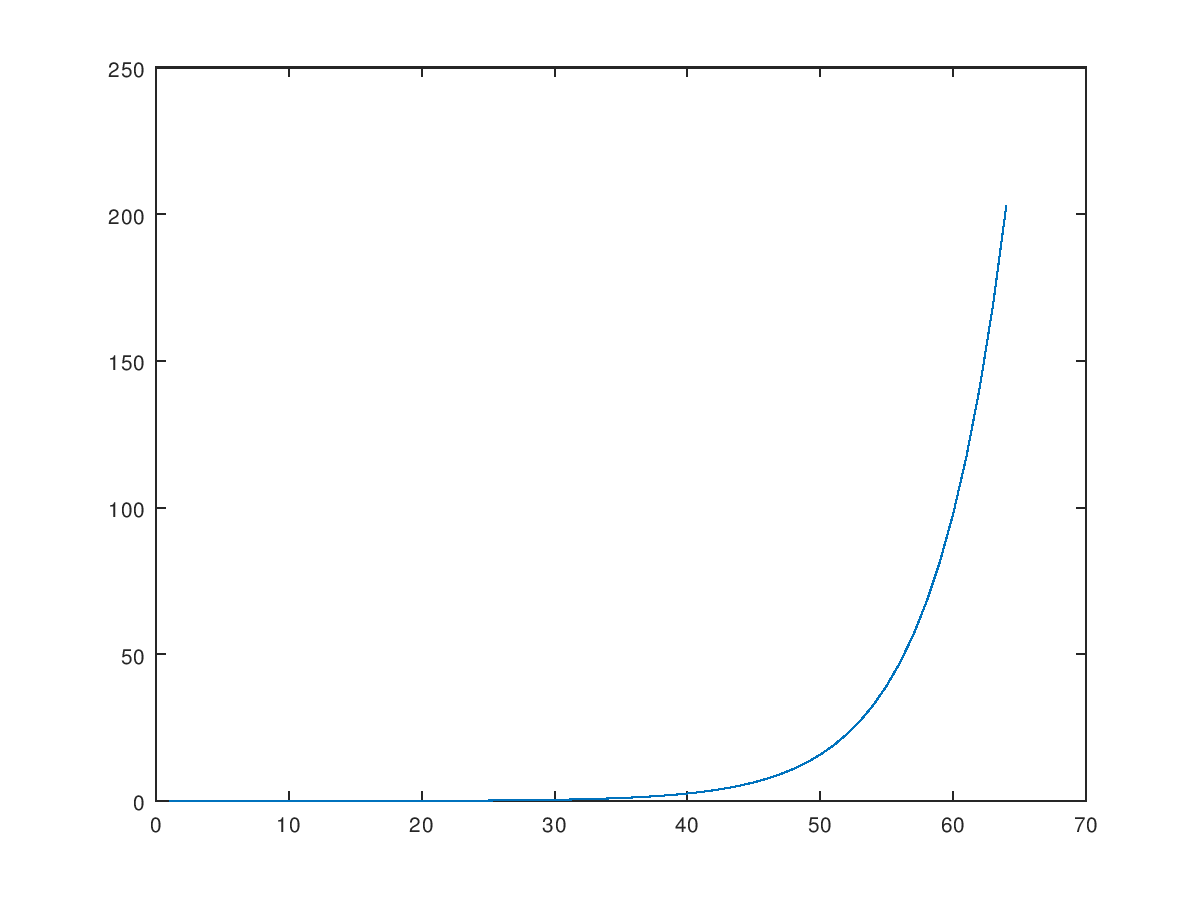
\includegraphics[width=5cm]{radiusSamples.png} }}%
    \subfloat[ $\rho$ samples]{{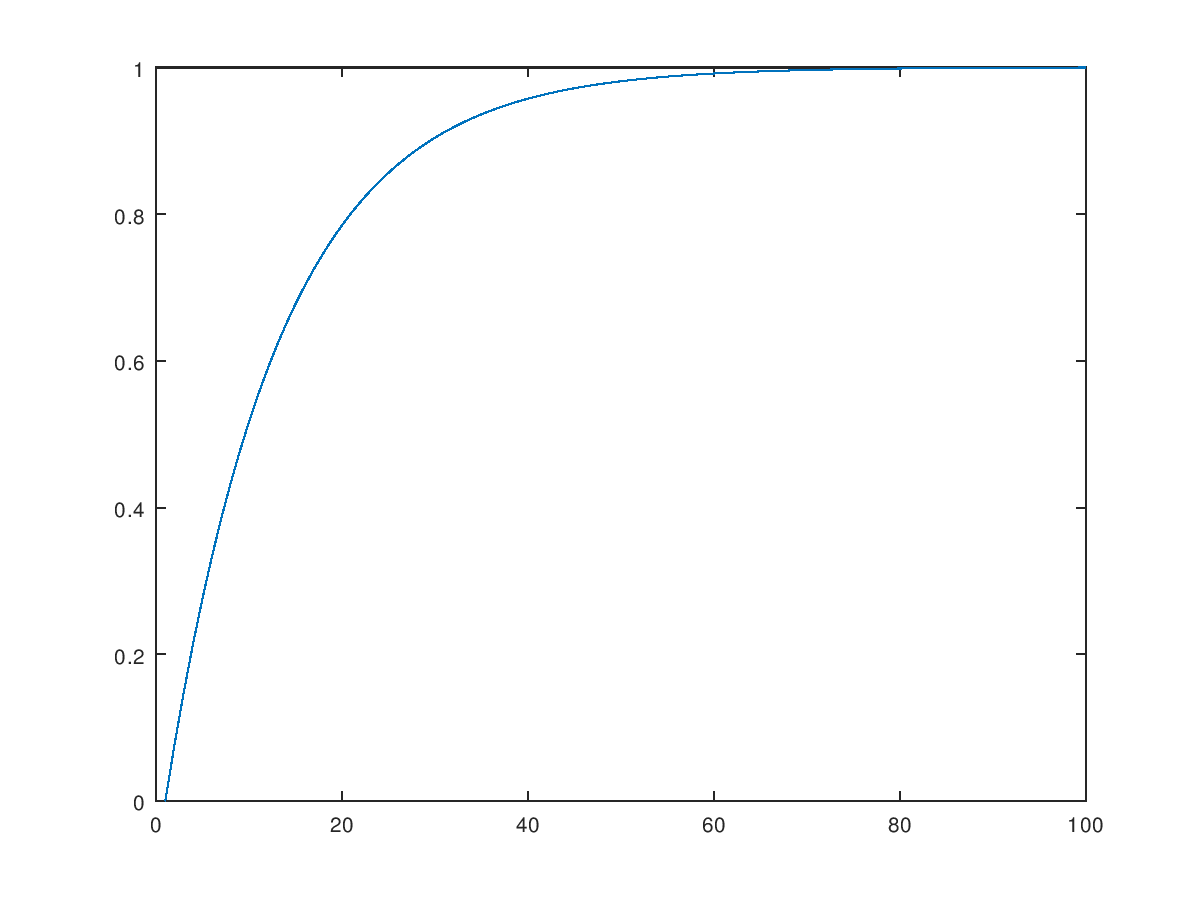
\includegraphics[width=5cm]{rhoSamples.png} }}%
    \subfloat[ $\rho_{eff}$ samples]{{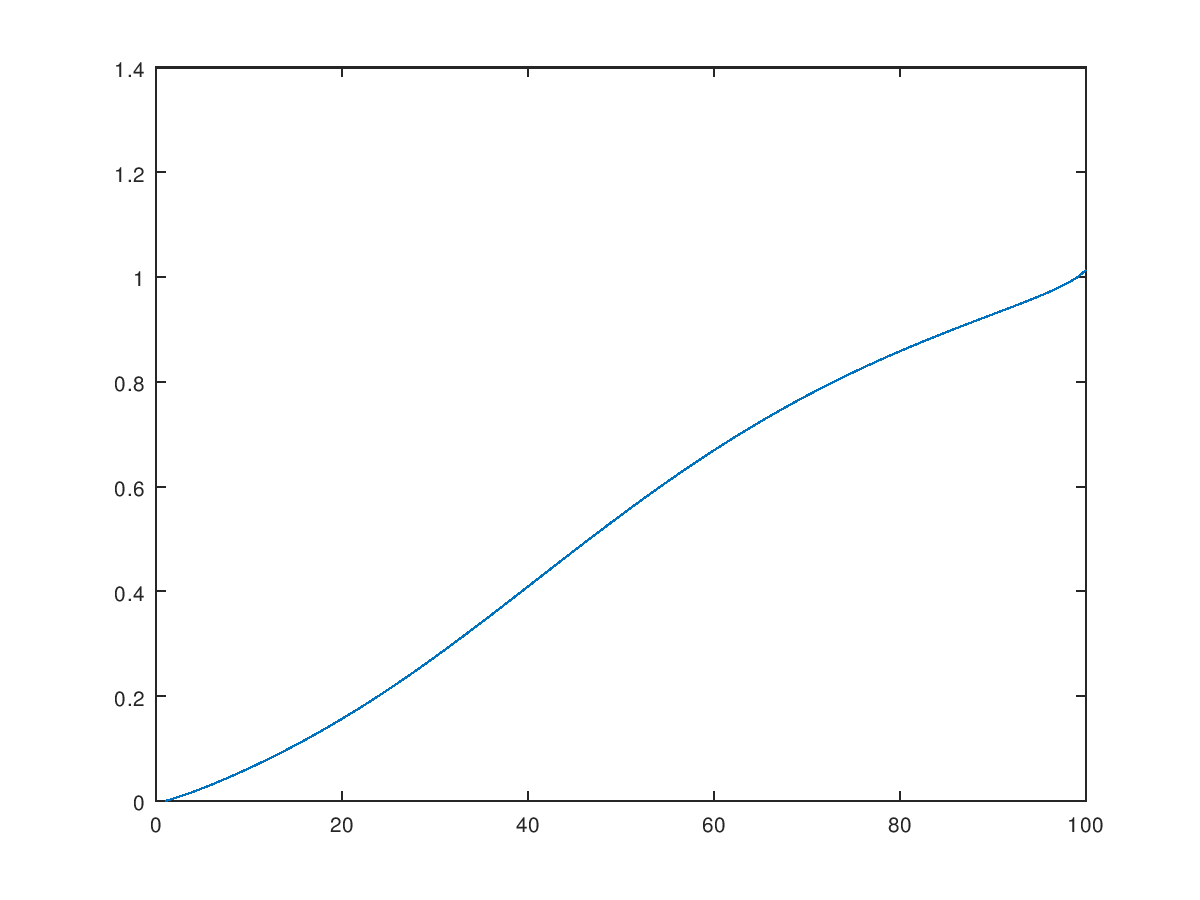
\includegraphics[width=5cm]{rhoEffSamples.png} }}%
    \caption{}%
    \label{fig:example}%
\end{figure}

\begin{figure}[H] 
        \centering 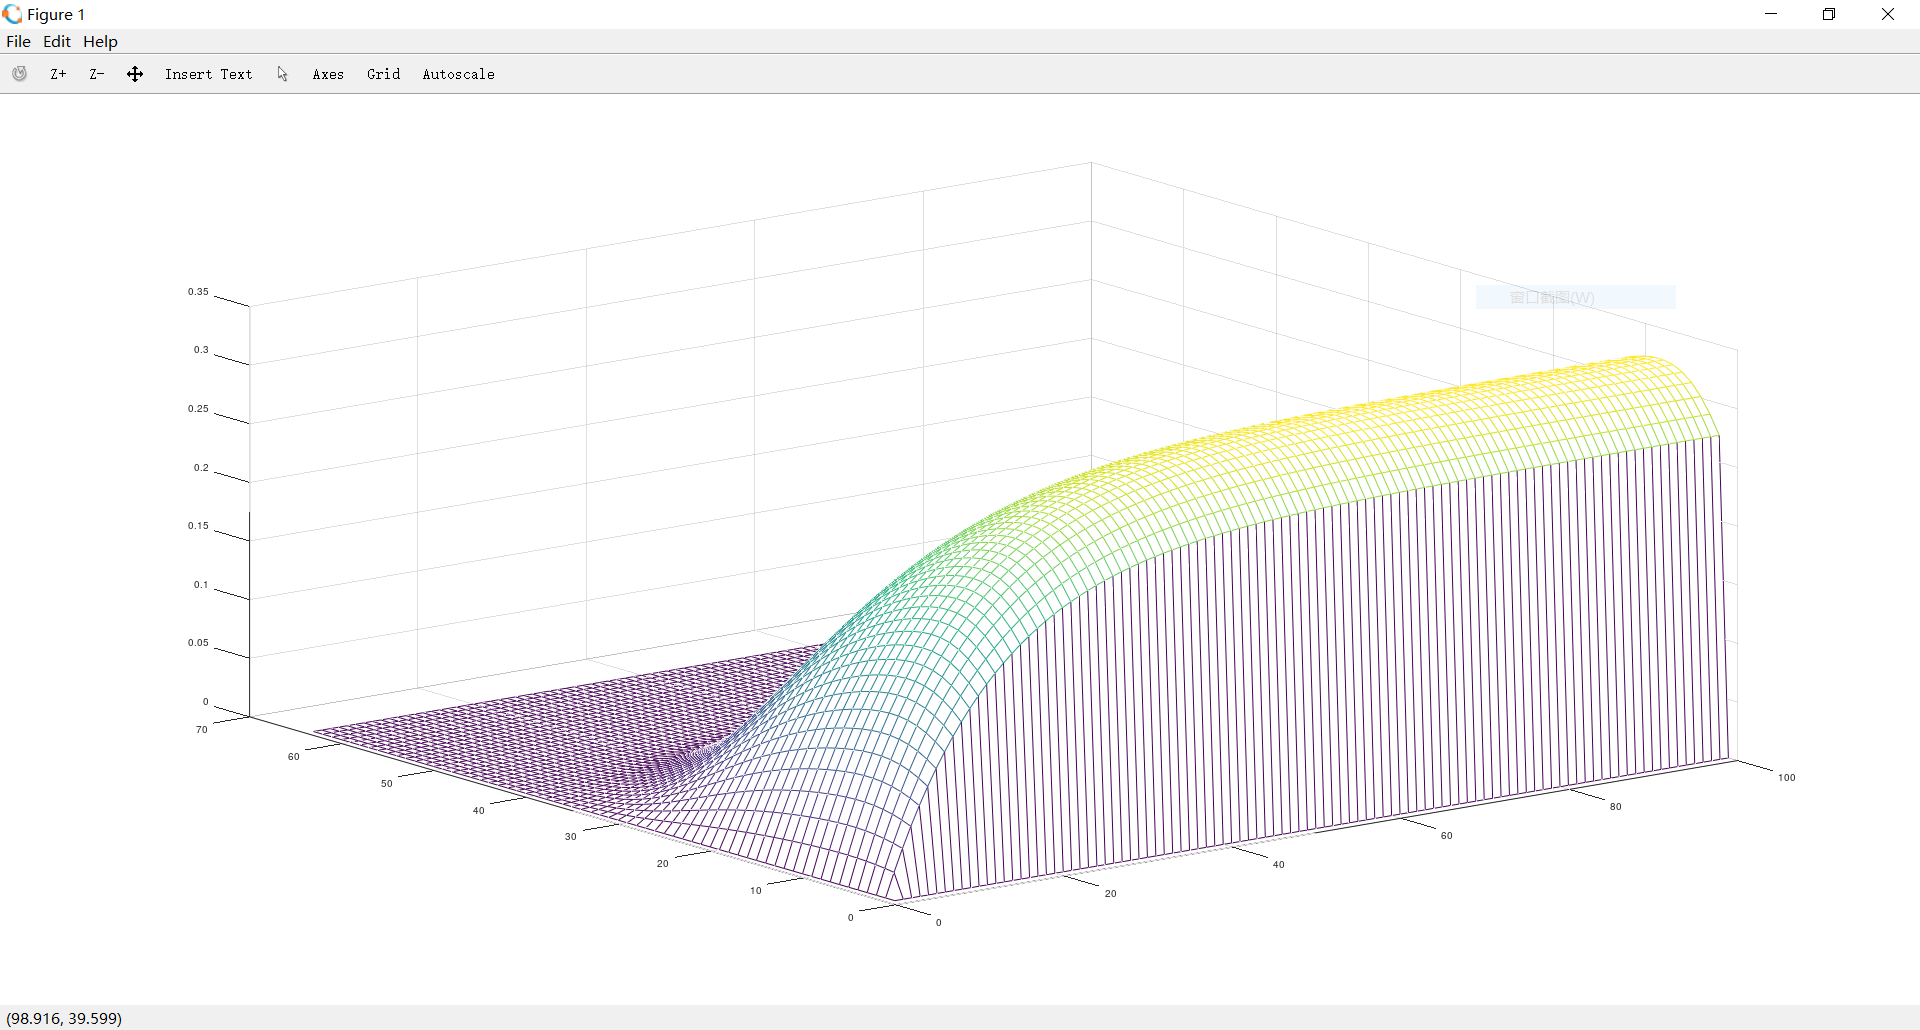
\includegraphics[width=0.8\columnwidth]{profile.png}
        \caption{\label{fig:profile}PBD profile $S_r(radius, \rho)$}
\end{figure}

\subsection{Model II: Sum of Exponentials}

The profile $R(r:radius, A:\rho_{Eff})$ is approximated by equation:

\begin{equation}
    R(r, A) = A\frac{e^{-r/d} + e^{-r/(3d)}}{8\pi dr}
\end{equation}

where we set the parameter $d$ as $d = s / l$ and $l$ is the mean free path. $s$ is a parameter used to approximate the profile in different configurations: search light or diffuse. In my implementation, search light configuration is used. So the equation becomes

\begin{equation}
    R(r, A) = A s \frac{e^{-sr/l} + e^{-sr/(3l)}}{8\pi lr}
\end{equation}

where

\begin{equation}
    s = 1.85-A+7|A-0.8|^3
\end{equation}

The cdf is calculated by integrating the profile on the disk and the albedo is canceled.

\begin{equation}
    cdf(r) = 1 - \frac{1}{4} e^{-r/d} - \frac{3}{4} e^{-r/(3d)}
\end{equation}

The cdf is not analytically invertible. The SoE paper suggests three methods\cite{christensen2015approximate} and I choose the MIS method which should be the fastest method for GPU computing. MIS has fixed number of operation without extra memory requirement. The other two methods are Newton steps and look-up table. Newton steps has a unstable loop which will slow down all threads in GPU. Look-up table needs extra memory. The drawback of MIS is that the variance will increase which means each sample will have less contribution to the converged value. However, the speed gain with MIS computing in GPU comparing to Newton steps and look-up table should overcome the sampling ineffectiveness.

\section{Sampling methods}

\subsection{CUDA GPU Path Tracing}

GPU computing efficiency requires different thinking model from CPU computing's. The computing follows SIMD (single instruction multiple data) or specifically SIMT (single instruction multiple threads) in CUDA computing. The best case for SIMT is that the same operations need to be performed on a large set of threads/data and the operations don't have dependencies on other threads/data. Typically 32 threads are grouped together into one warp and the instruction is lock-stepped in a warp\cite{han2011hicuda}. Path tracing is suitable to GPU computing since each pixel's data is independent and the operation on each pixel is similar. 

The speed limitation happens when there are totally different material calculations or different branches in a same material, which we call branch/thread divergence. The uncertain loop time will also be a problem since all the threads in a warp need to wait for the single thread with the longest loop time. GPU computing also has more resource limitation than CPU, such as limited device memory and limited bandwidth.

I use an open-source CUDA BVH\cite{aila2012understanding} developed by Nvidia and altered the BVH to support more mesh attributes. It's worth mentioning that a well-optimized BVH for the Nvidia's hardware should result in a huge speed up for the path tracing program. So the partial credits of the efficiency of my renderer goes to Nvidia's hardware and BVH software supporting. It's a separate area from rendering algorithms and sampling methods where I focus on.

\subsection{Sampling Algorithm}

In this section we denote where the eye ray goes in the surface as $p_i$ and where the eye ray goes out the surface as $p_o$.

\subsubsection{Step 1, Sample a probe ray}

The algorithm first samples a radius $r$ according to the profile distribution. And then it calculates a maximum radius $r_{max}$ (0.999 for uniform random input). Then it calculates a perpendicular probe ray (has the same direction as surface normal at $p_i$) to find the intersection with the surface as the point where the ray goes out as shown in Figure \label{fig:probe}. The $p_o$ in the figure is defined as where eye ray goes in the surface, or where the light ray goes out the surface. The $p_i$ is defined as where eye ray goes out the surface, or where the light ray goes in the surface. $n_o$ is the normal at $p_o$. The $p_i,p_o,n_o$ in the figure have different meanings to all the other $p_i, p_o$ in this section. The figure is referenced from \cite{pharr2016physically}.

\begin{figure}[H] 
        \centering 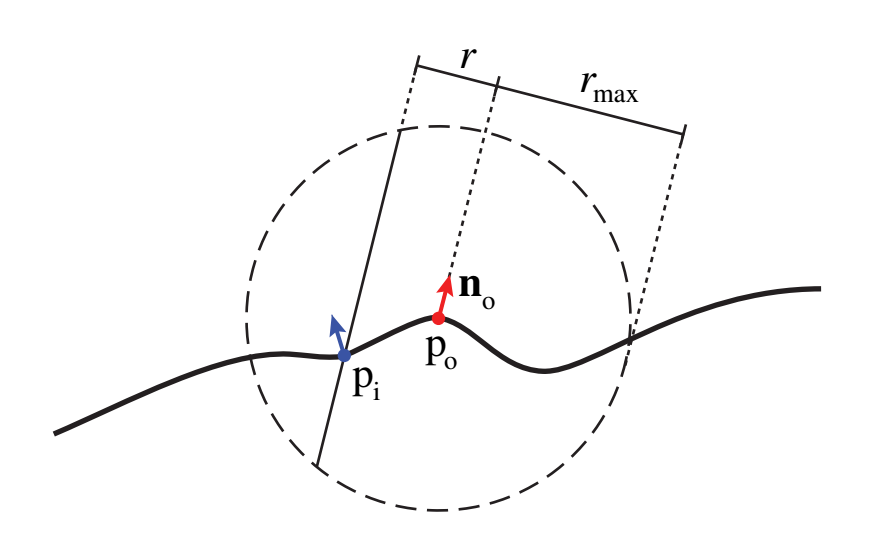
\includegraphics[width=0.8\columnwidth]{probeRay.png}
        \caption{\label{fig:probe}Sampling probe ray}
\end{figure}

The sampling requires the inverse of the cdf of the profile. PBD samples with Catmull-Rom 2D method using a look-up table. SoE calculates the inverse of cdf of two distribution using MIS method. The probe ray has 50\% chance to have the same direction as surface normal, 25\% each for tangent and bi-tangent directions. This will increase the overall variance but effectively reduce the variance at geometries with steep angle.

\subsubsection{Step 2, Probe ray scene intersection}

The ray scene intersection calculation is the computing bottleneck here so we want minimum probes to increase speed while we still get a good sample. The algorithm allows a user to set a loop count instead of its counterpart in the CPU algorithm, which is a endless loop with a termination condition. CPU algorithm also uses an array or a linked list to record all potential $p_o$ and randomly choose one of them after the probing.

The novelties of my method are:
\begin{itemize}
    \item I adopt reservoir sampling, which is a on-line algorithm to use a random number to test if it keeps the old $p_o$ record or adopts a new record $p_o$ each time it finds a new valid $p_o$ candidate. The possibility to adopt a new candidate is one over the number of candidates. For example, the first candidate has the chance of $\frac{1}{1}=100\%$ to be chosen, the second has the chance $\frac{1}{2}=50\%$ and the third has $\frac{1}{3}=33.3\%$, for three candidates in total, the chance for the first one being chosen is $(1-\frac{1}{2})\times(1-\frac{1}{3}) = \frac{1}{3}=33.3\%$ so the sampling is uniform.
    \item I fix the number of loops while the probe ray scene intersection count is recorded. The number of intersections is important to correctly evaluate the pdf since the chance of choosing every intersection is equal so the pdf needs to divide the intersection count. However, a correct intersection count needs infinite loops rather than a fixed number of loops since it's possible a probe ray intersects a scene for larger number of times then the fixed loop number. So my method has bias to the infinite loops method. While in the real application cases, the case when a ray intersects with more surfaces than the fixed loop number is rare and the fixed loop number is defined by the user. The user controls the fixed loop number and it's a quality-speed trade-off.
\end{itemize}
Using this method, I effectively fix the number of loops and reduce the memory usage, which will lead to a computing speedup.

In this step, the algorithm also makes sure that the new hit point $p_o$ is on the same surface with the old hit point $p_i$. For a large scene with multiple subsurface scattering materials, object id is needed. Currently it only checks the material id.

\subsubsection{Step 3, Sample next direction}

This step simply needs a cosine hemisphere sampling which is the same sampling method for Lambertian diffuse calculation. There should be more elaborate sampling method but the cosine hemisphere sampling is very fast and work without any problems.

\subsubsection{Step 4, Calculate the color mask}

Color mask is calculated with the profile function. For PBD, It reads the value from the loop-up table and performs a few steps of interpolations. For SoE, MIS calculation is performed. Then we need to calculate the pdf carefully since the probe ray sampling involves a lot of steps.

\subsubsection{Step 5, Calculate direct light contribution}

For distant lighting, the light contribution from a single direction so the randomly sampled next ray direction will impossibly hit the lighting direction. MIS is used to calculate the direct light contribution with surface BRDF, surface pdf and lighting pdf. The lighting pdf in the distant lighting case is constant.

\subsubsection{Sampling Algorithm Analysis}

The overall sampling method brings thread coherency and reduces memory usage in contrast to sampling method used in CPU subsurface scattering. The advantage is the algorithm runs faster on GPU and user can define the max loop count to control the rendering quality. The downside is the sampling has a very small chance to fail. In CPU method, it is possible the program will loop for a infinite time until it finds a good sample, which means given a fixed loop time the algorithm has a chance to fail. This will lead to a little bias and a higher variance in the result. The good thing is that the speed advantage can overcome the variance issue. The bias issue is a real limitation of the sampling method. However it's almost no visual difference between the rendering result so the small bias shouldn't be a real issue.

\section{Evaluation}

The evaluation is performed on a machine with Intel i7-6700 CPU and Nvidia GTX 960M GPU. The path tracings allow 3 max bounces and no Russian Roulette. The resolution is 720x720. I run the path tracing on pbrt-v3 CPU renderer and my GPU renderer. There are three rendering methods: CPU PBD in pbrt-v3, GPU PBD and GPU SoE. I tested the three methods in three different scenes for three different time limits. The goal is to show that all three methods can generate similar result while my GPU methods are less noisy which means they run faster.

The scale factor only affects the spatial scale of the object or the concentration of the media. I adjust the scale factor freely to match the real life object size and media concentration. The scale factor is different for pbrt-v3 and my GPU renderer.

The albedo and the mean free path for the renderings are also different. I adjusted them to achieve similar results among all rendering methods. Physically, same albedo with same mean free path should result in same rendering. However pbrt-v3 and my renderer have different assumptions and approximation for the physical parameters. pbrt-v3 uses 7-channel SPD color while I use 3-channel RGB color which will affect the sampling range of the result since the sampling distance is decided by each channel. Typically, every renderer has its own personality and its own logic for its parameters, even it's "physically based". The same scene rendered by Disney's and Pixar's renderer result in total different pictures. So the goal is not to render the strictly physically based image but to render the perceptually similar visuals. 

\subsection{Flat Slab Beam Lighting Test}

A flat slab with a perpendicular small beam of light scene is a basic test scene for subsurface scattering materials. The profile of subsurface scattering can be visualized and the correctness of implementation can be verified visually.

\begin{figure}[H]
    \centering
    \subfloat[5 seconds]{{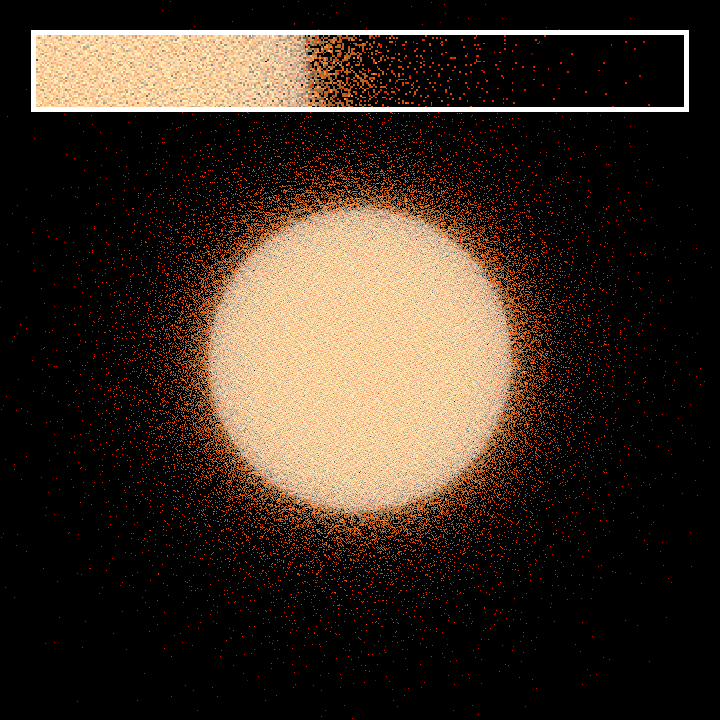
\includegraphics[width=5cm]{pbrt-5.png} }}%
    \subfloat[50 seconds]{{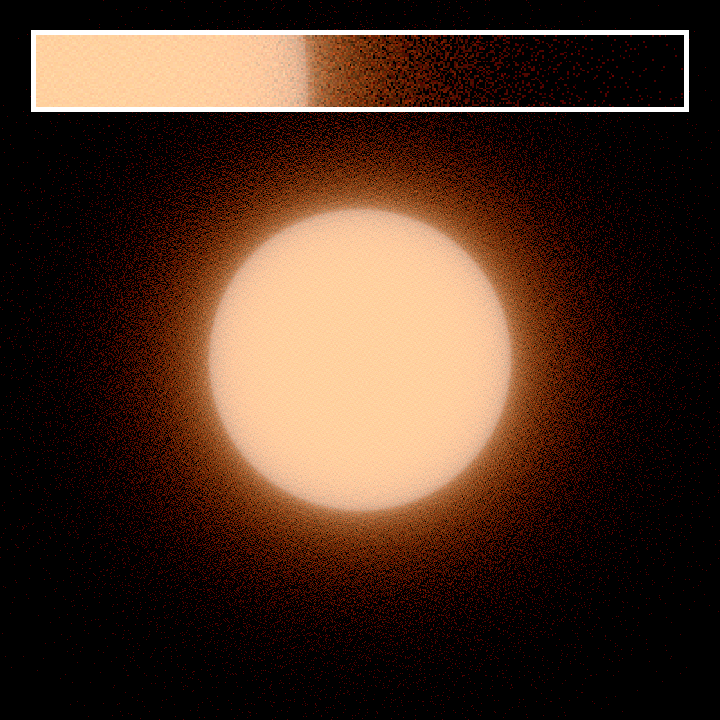
\includegraphics[width=5cm]{pbrt-50.png} }}%
    \subfloat[500 seconds]{{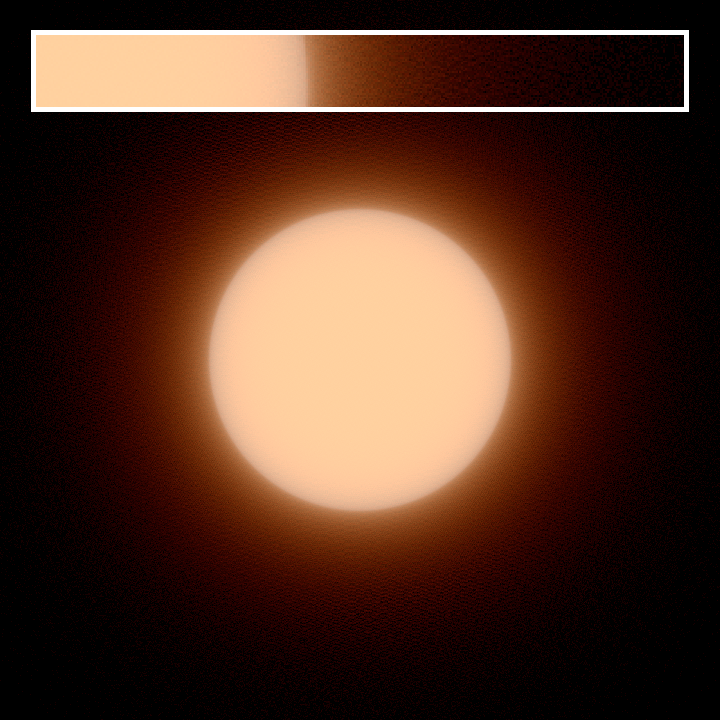
\includegraphics[width=5cm]{pbrt-500.png} }}%
    \caption{pbrt-v3 (CPU PBD)}%
    \label{}%
\end{figure}

\begin{figure}[H]
    \centering
    \subfloat[5 seconds]{{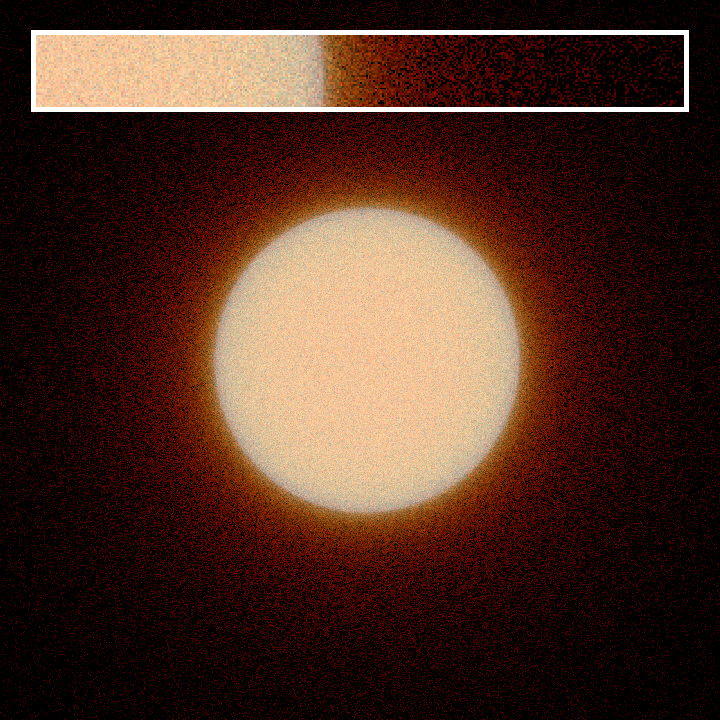
\includegraphics[width=5cm]{pbd-5.png} }}%
    \subfloat[50 seconds]{{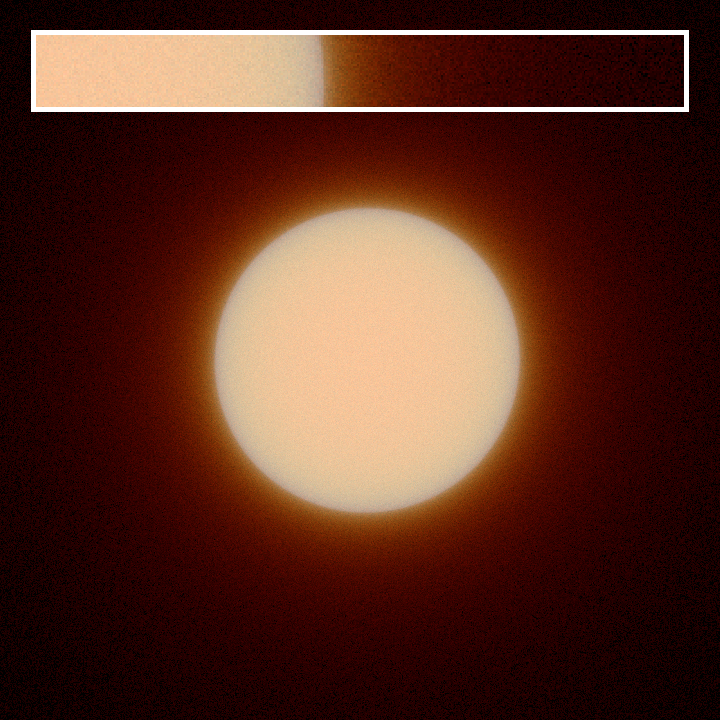
\includegraphics[width=5cm]{pbd-50.png} }}%
    \subfloat[500 seconds]{{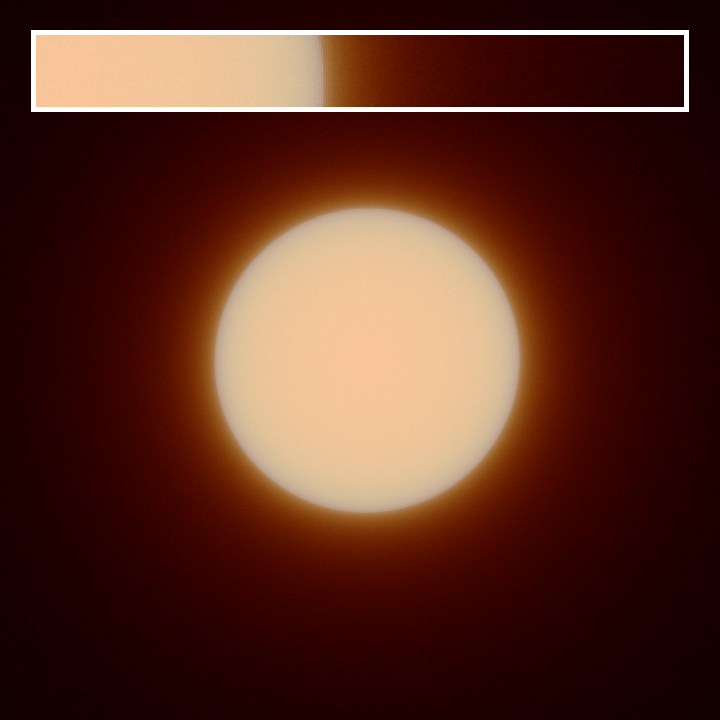
\includegraphics[width=5cm]{pbd-500.png} }}%
    \caption{GPU PBD}%
    \label{}%
\end{figure}

\begin{figure}[H]
    \centering
    \subfloat[5 seconds]{{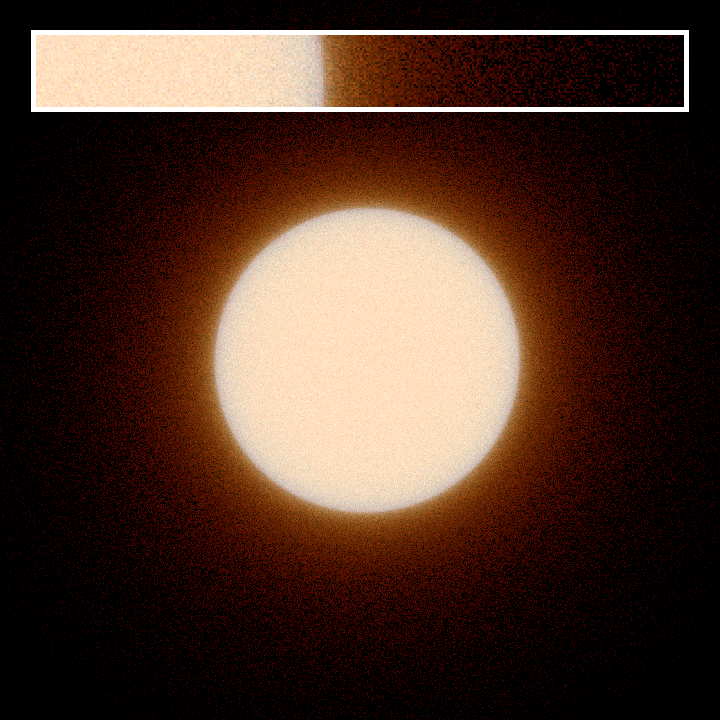
\includegraphics[width=5cm]{soe-5.png} }}%
    \subfloat[50 seconds]{{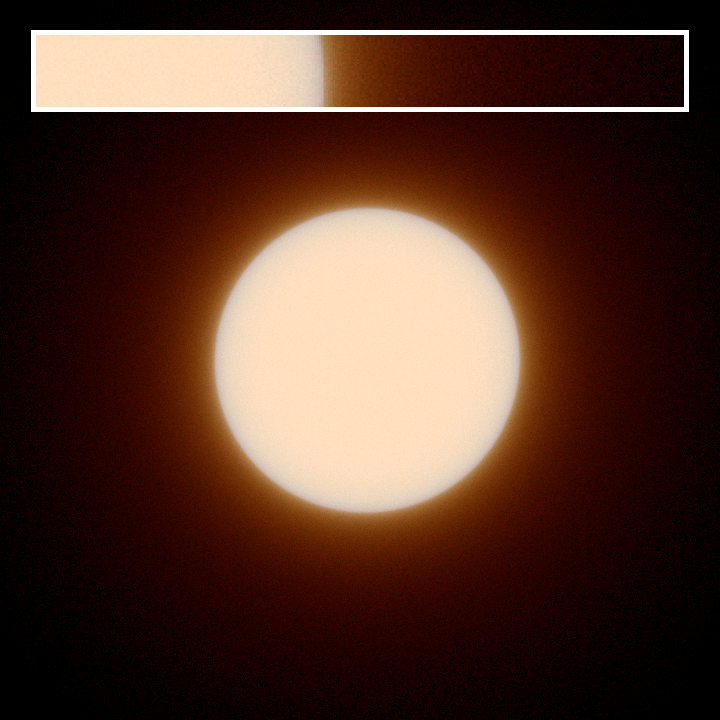
\includegraphics[width=5cm]{soe-50.png} }}%
    \subfloat[500 seconds]{{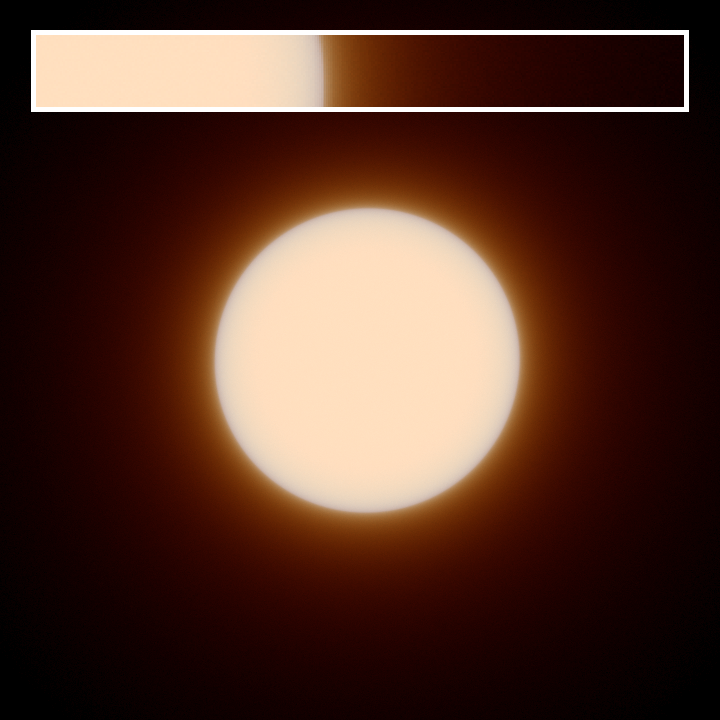
\includegraphics[width=5cm]{soe-500.png} }}%
    \caption{GPU SoE}%
    \label{}%
\end{figure}

We see from the images that the well-known pbrt-v3 CPU rendering is noisier then my GPU implementations. pbrt-v3 is about 10 times slower than the GPU PBD. The GPU SoE runs about 3 times faster than the GPU PBD. pbrt-v3 should produce the most accurate rendering since it's based on physics more strictly. My implementations have more approximations. However it is almost impossible to tell which one is more physically accurate just using our eyes.

\subsection{Complex Geometry Distant Lighting Test}

A complex-shaped geometry with a distant lighting illuminated from the backside of the geometry scene can show that the object is translucent. We can test any rendering methods or translucent materials perceptually with this scene setting.

\begin{figure}[H]
    \centering
    \subfloat[10 seconds]{{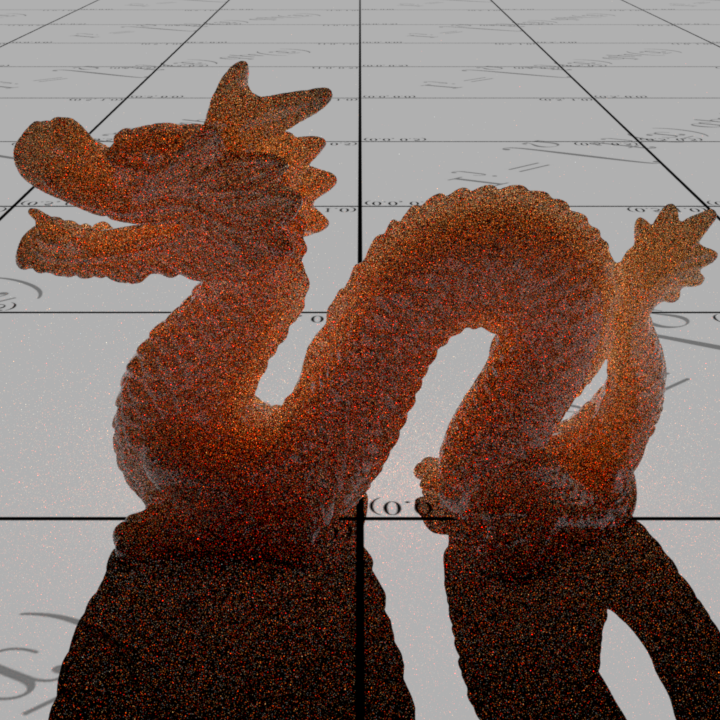
\includegraphics[width=5cm]{pbrt-10.png} }}%
    \subfloat[100 seconds]{{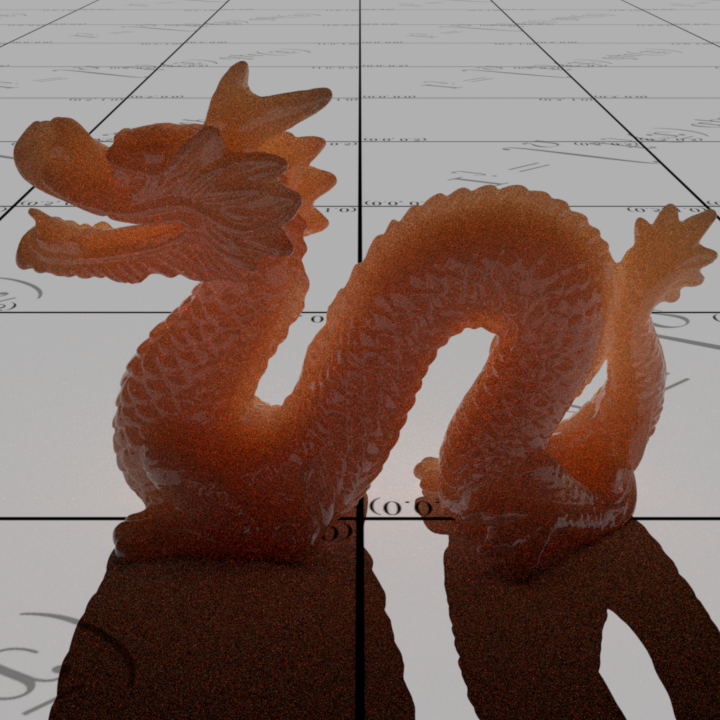
\includegraphics[width=5cm]{pbrt-100.png} }}%
    \subfloat[1000 seconds]{{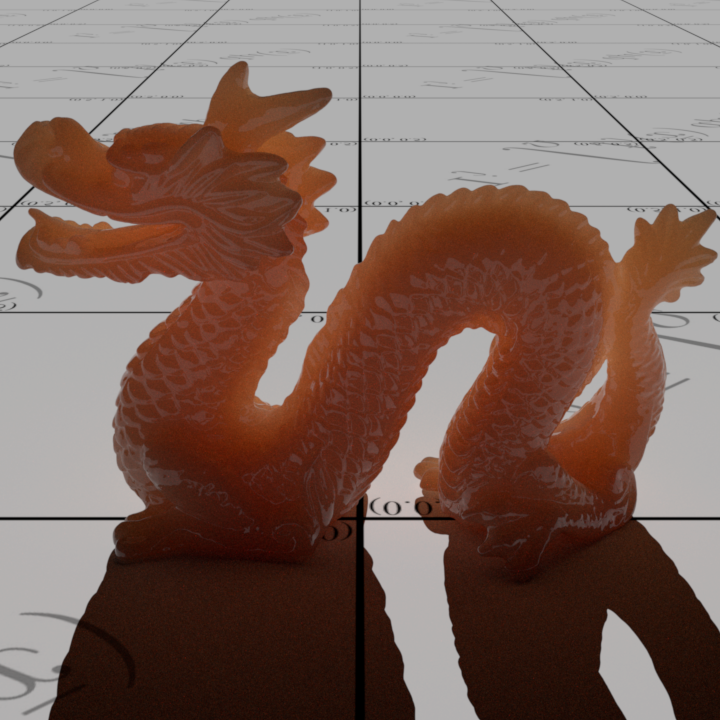
\includegraphics[width=5cm]{pbrt-1000.png} }}%
    \caption{pbrt-v3 (CPU PBD)}%
    \label{}%
\end{figure}

\begin{figure}[H]
    \centering
    \subfloat[10 seconds]{{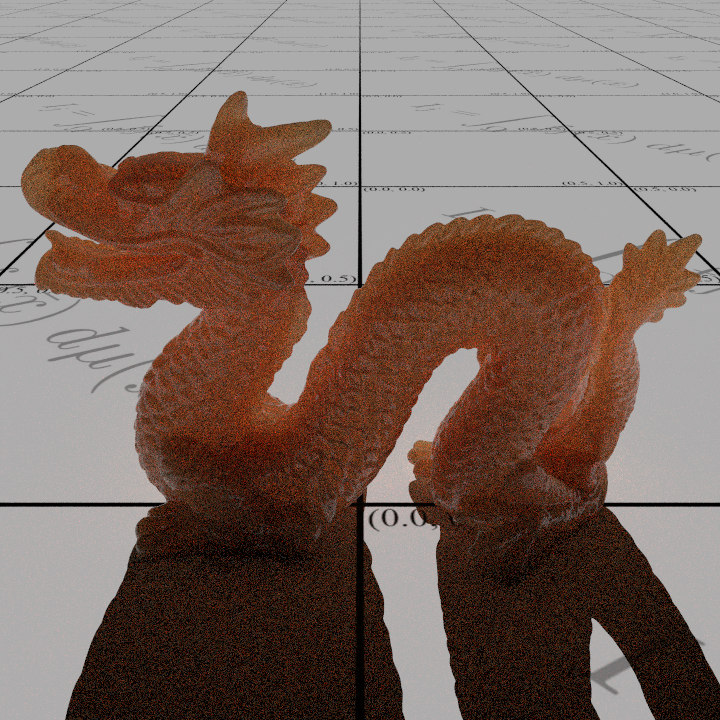
\includegraphics[width=5cm]{pbd-10.png} }}%
    \subfloat[100 seconds]{{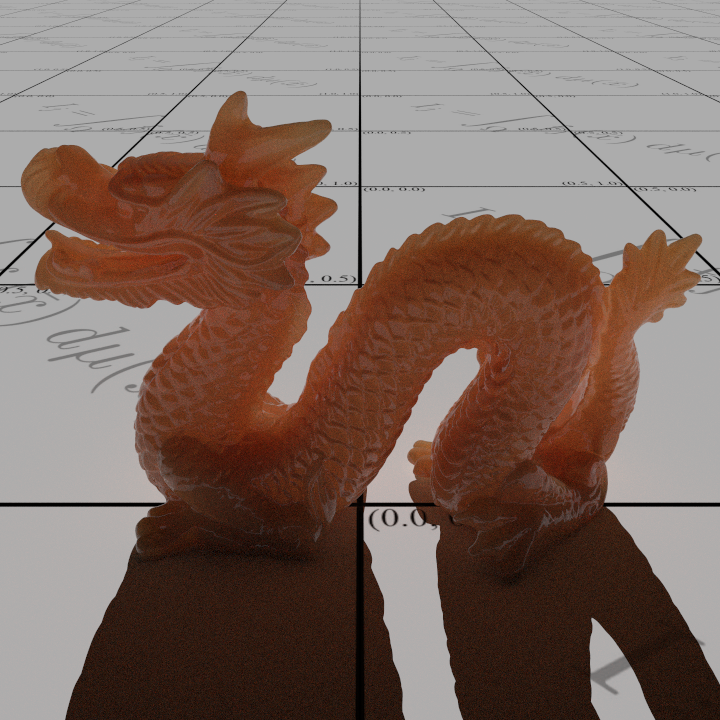
\includegraphics[width=5cm]{pbd-100.png} }}%
    \subfloat[1000 seconds]{{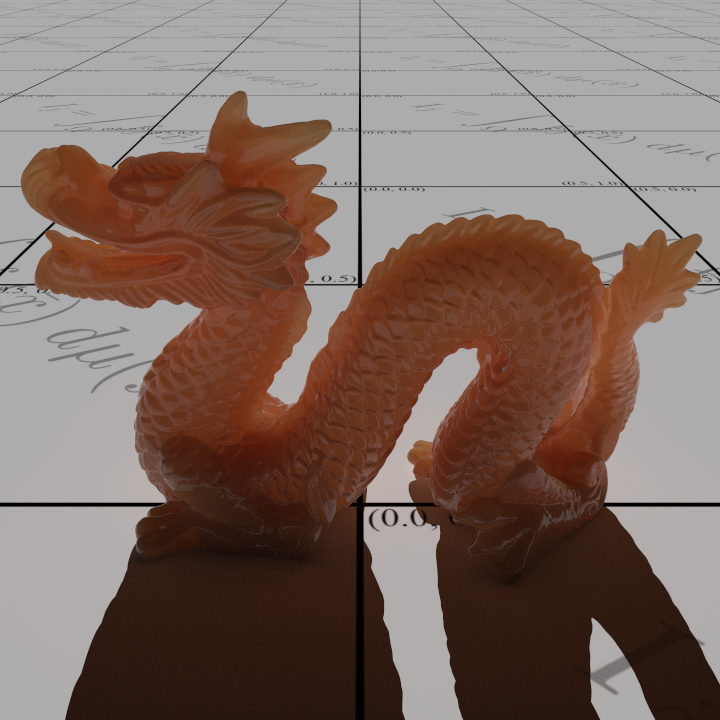
\includegraphics[width=5cm]{pbd-1000.png} }}%
    \caption{GPU PBD}%
    \label{}%
\end{figure}

\begin{figure}[H]
    \centering
    \subfloat[10 seconds]{{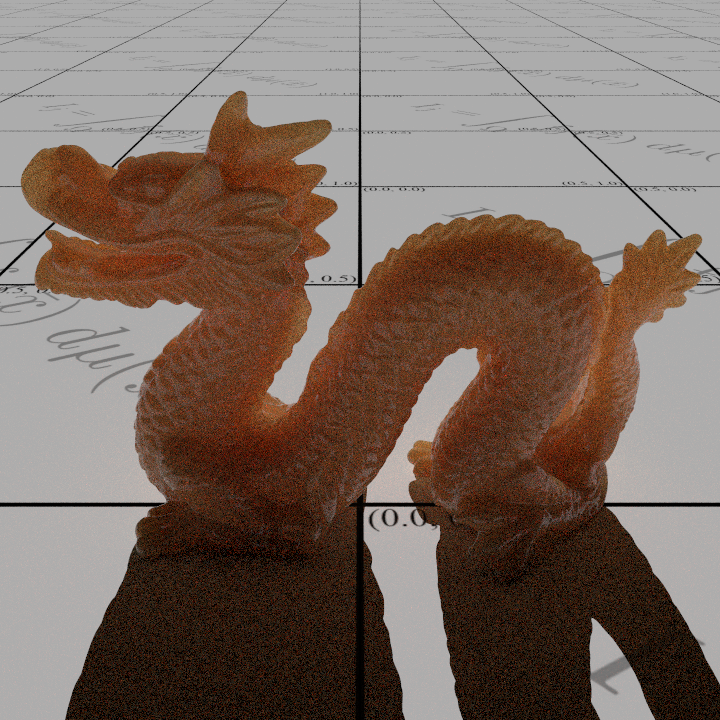
\includegraphics[width=5cm]{soe-10.png} }}%
    \subfloat[100 seconds]{{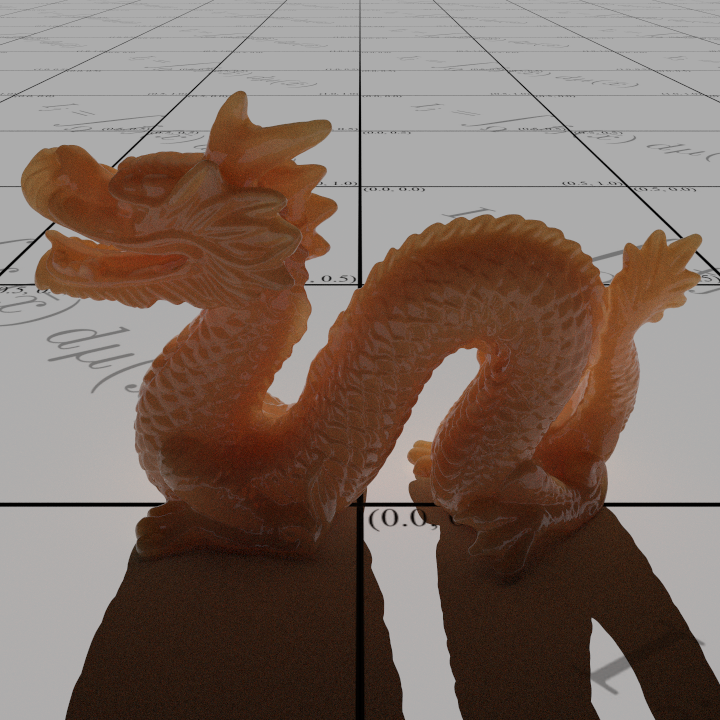
\includegraphics[width=5cm]{soe-100.png} }}%
    \subfloat[1000 seconds]{{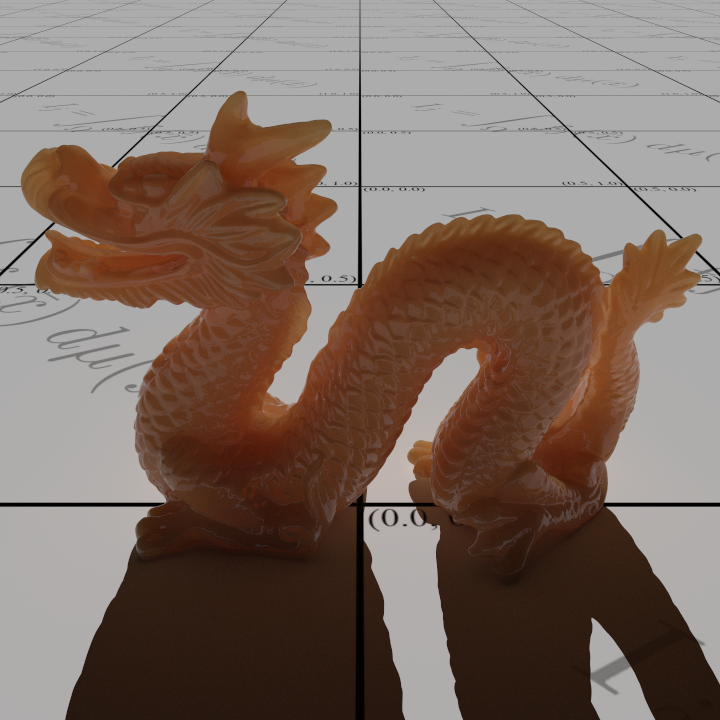
\includegraphics[width=5cm]{soe-1000.png} }}%
    \caption{GPU SoE}%
    \label{}%
\end{figure}

We see that all three methods render the same color variation. From the thin part to the thick part of the geometry, the color changes from light yellow to orange to red and then fade to black. GPU PBD and SoE are less noisy.

\subsection{Human Face Environmental Lighting Test}

A human head model with a natural environmental lighting scene is an application facing setting. The movie "The Matrix Reloaded" uses a similar scene setting to render the fighting scene and the skin rendering looks so natural that we can hardly tell that the characters are actually renderings\cite{borshukov2005realistic}.

\begin{figure}[H]
    \centering
    \subfloat[5 seconds]{{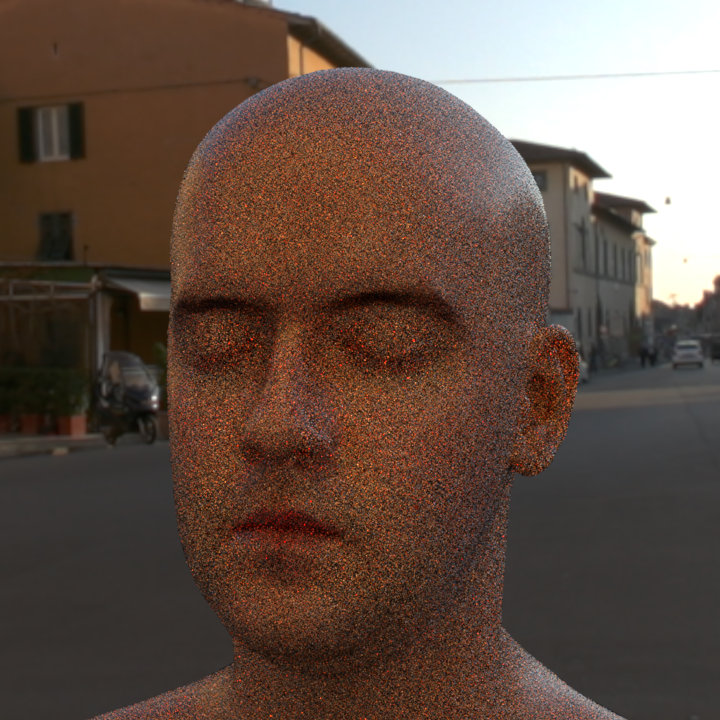
\includegraphics[width=5cm]{t3-pbrt-5.png} }}%
    \subfloat[50 seconds]{{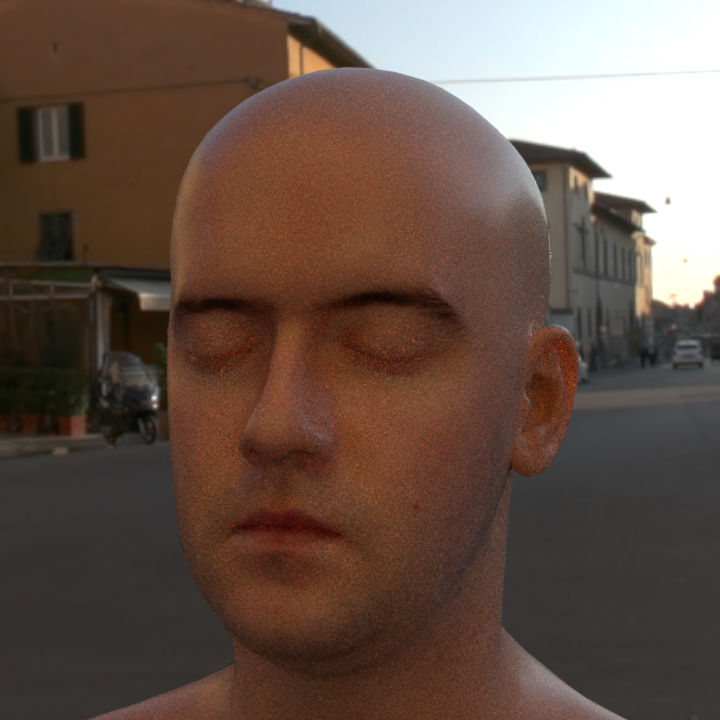
\includegraphics[width=5cm]{t3-pbrt-50.png} }}%
    \subfloat[500 seconds]{{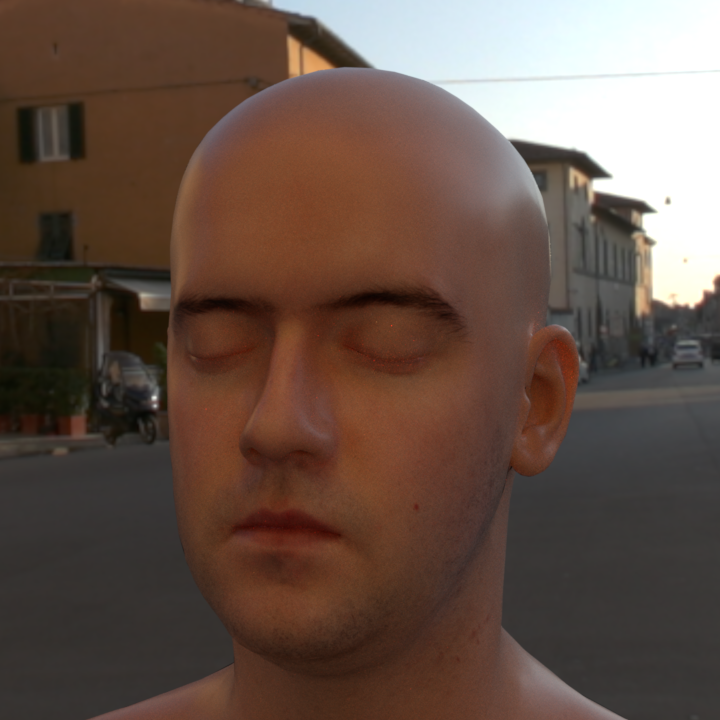
\includegraphics[width=5cm]{t3-pbrt-500.png} }}%
    \caption{pbrt-v3 (CPU PBD)}%
    \label{}%
\end{figure}

\begin{figure}[H]
    \centering
    \subfloat[5 seconds]{{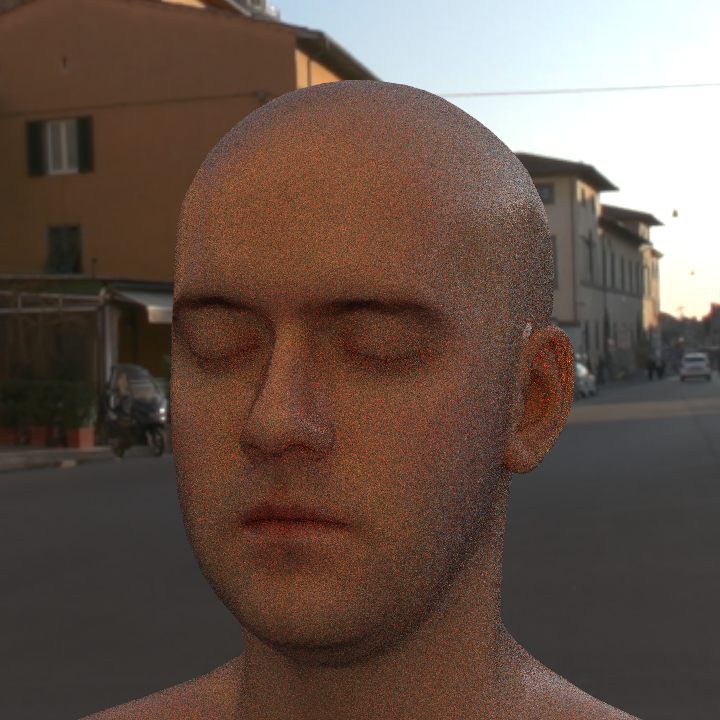
\includegraphics[width=5cm]{t3-pbd-5.png} }}%
    \subfloat[50 seconds]{{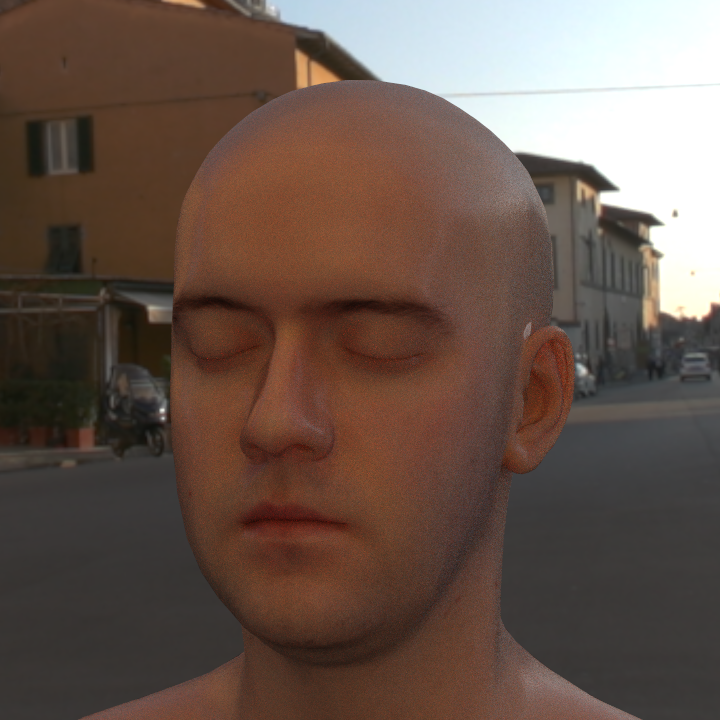
\includegraphics[width=5cm]{t3-pbd-50.png} }}%
    \subfloat[500 seconds]{{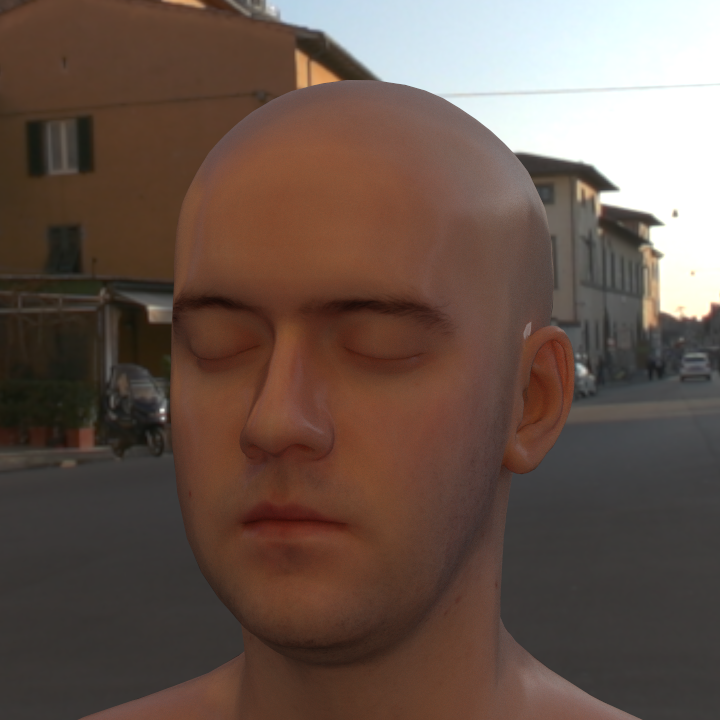
\includegraphics[width=5cm]{t3-pbd-500.png} }}%
    \caption{GPU PBD}%
    \label{}%
\end{figure}

\begin{figure}[H]
    \centering
    \subfloat[5 seconds]{{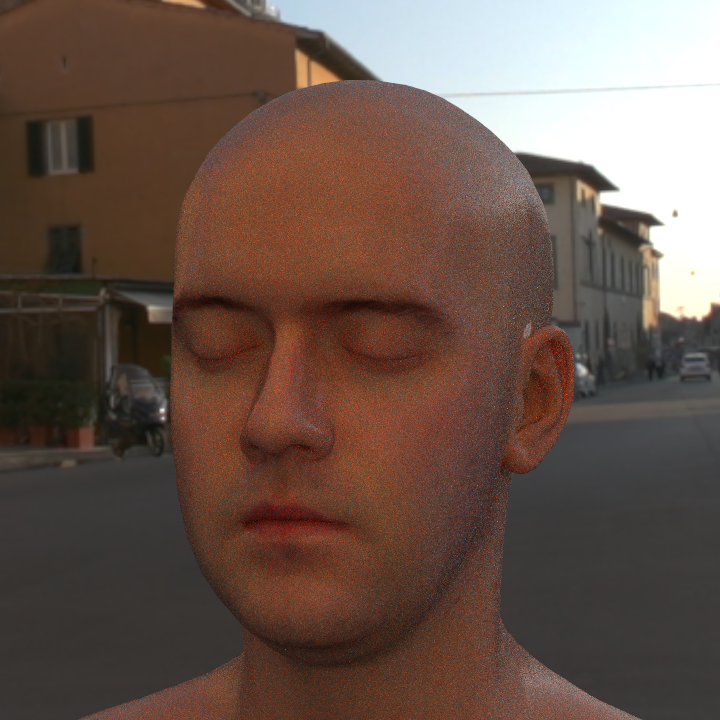
\includegraphics[width=5cm]{t3-soe-5.png} }}%
    \subfloat[50 seconds]{{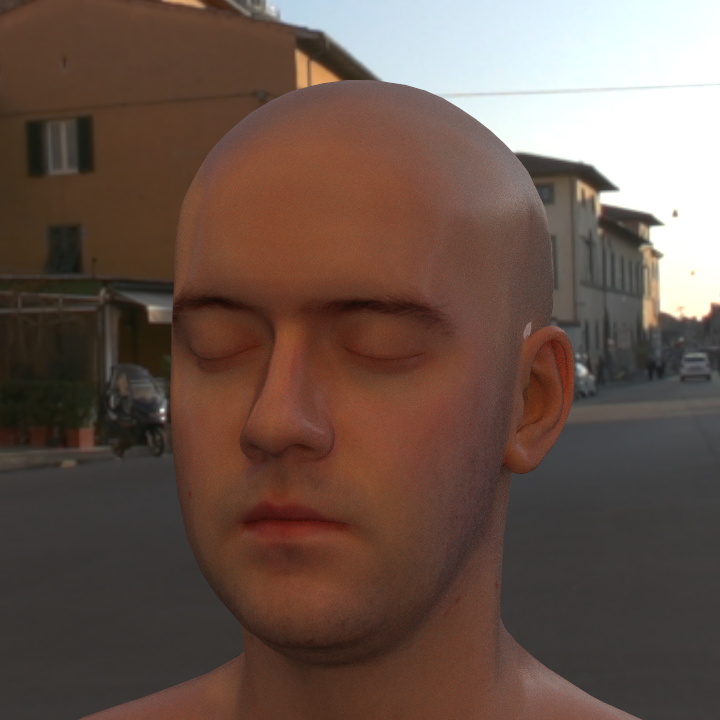
\includegraphics[width=5cm]{t3-soe-50.png} }}%
    \subfloat[500 seconds]{{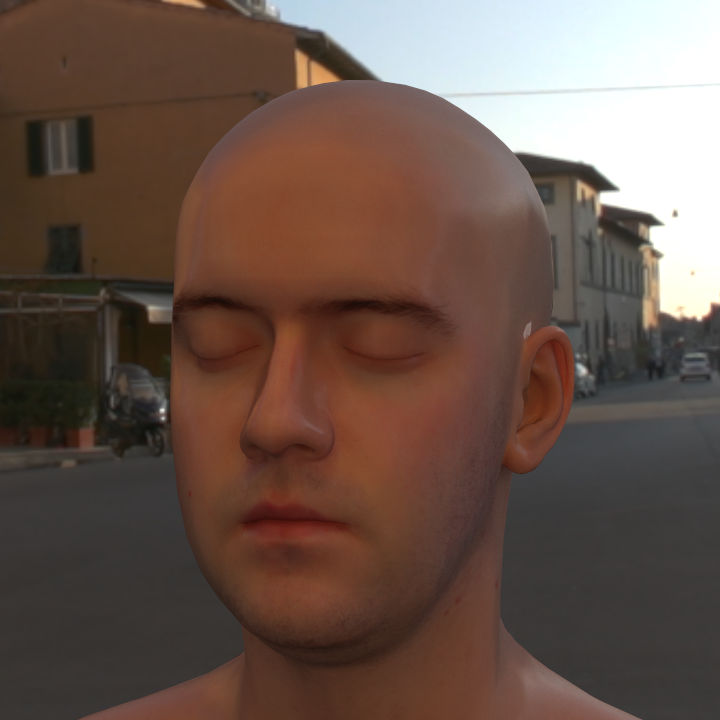
\includegraphics[width=5cm]{t3-soe-500.png} }}%
    \caption{GPU SoE}%
    \label{}%
\end{figure}

The facial region should appear soft and the ear should look transparent and have a red tint as it should look like in real life. All three methods can achieve this looking while GPU BPD and SoE are less noisy.

\subsection{Evaluation conclusions}

The beam plane test scene is simple to show the profile but hard to perceptually understand. The dragon scene shows the subsurface scattering perceptually and illustrates why we want this effect. The face scene is my goal but hard to evaluate so the other two scene are needed. The three test scenes show that the my implementation works and produces less noise.

\section{Conclusions}

Traditional human skin rendering using Monte Carlo volumetric path tracing is slow and needs too much computing power to be accurate. pbrt-v3 renders the human skin accurate but not enough efficient using CPU PBD. In this study, I devised a novel way of sampling for GPU based subsurface scattering rendering and implemented GPU PBD and GPU SoE rendering methods. After rendering tests with pbrt-v3, I have shown that my implementations are both efficient and accurate, which can be used to achieve efficient realistic human skin rendering.

The source codes of my renderer are on Github: https://github.com/wangkepfe/CUDA-Path-Tracing.

\bibliography{ref}{}
\bibliographystyle{plain}

\end{document}
